\chapter{Implementation and Solution}
\thispagestyle{fancy}

From the three specified refactorings, \textit{Toggle Function Definition} has 
been implemented in depth. This chapter explains how the refactoring was 
implemented and which problems had to be solved during development.

\section{Implementation approach}

At the beginning, as many cases as possible were collected on the project wiki 
to gain a view on what had to be realized, what was planned to take into scope 
and what had nothing to do with toggling function definitions. Some cases were 
simple, some exotic. The simplest one, toggling from inside a class to the same 
file outside the class, was chosen to be implemented first. 

Before that, a skeleton plugin was built with a NullRefactoring to try whether 
it was possible to develop a separate plugin instead of directly manipulating 
the CDT source code. By this approach it was assured that the developed plugin 
may be deployed easily even without being integrated into CDT.

After the first refactoring was implemented, more cases were added by priority. 

\section{Architecture}

In Eclipse, most of the architecture is already given. Some specialities of the 
toggle refactoring are presented in this section.

\subsection{Basic call flow}
The sequence diagram in figure %\ref{sd} illustrates the basic call flow when 
\textit{Toggle Function} is invoked.
\begin{figure}[h]
  \centering
  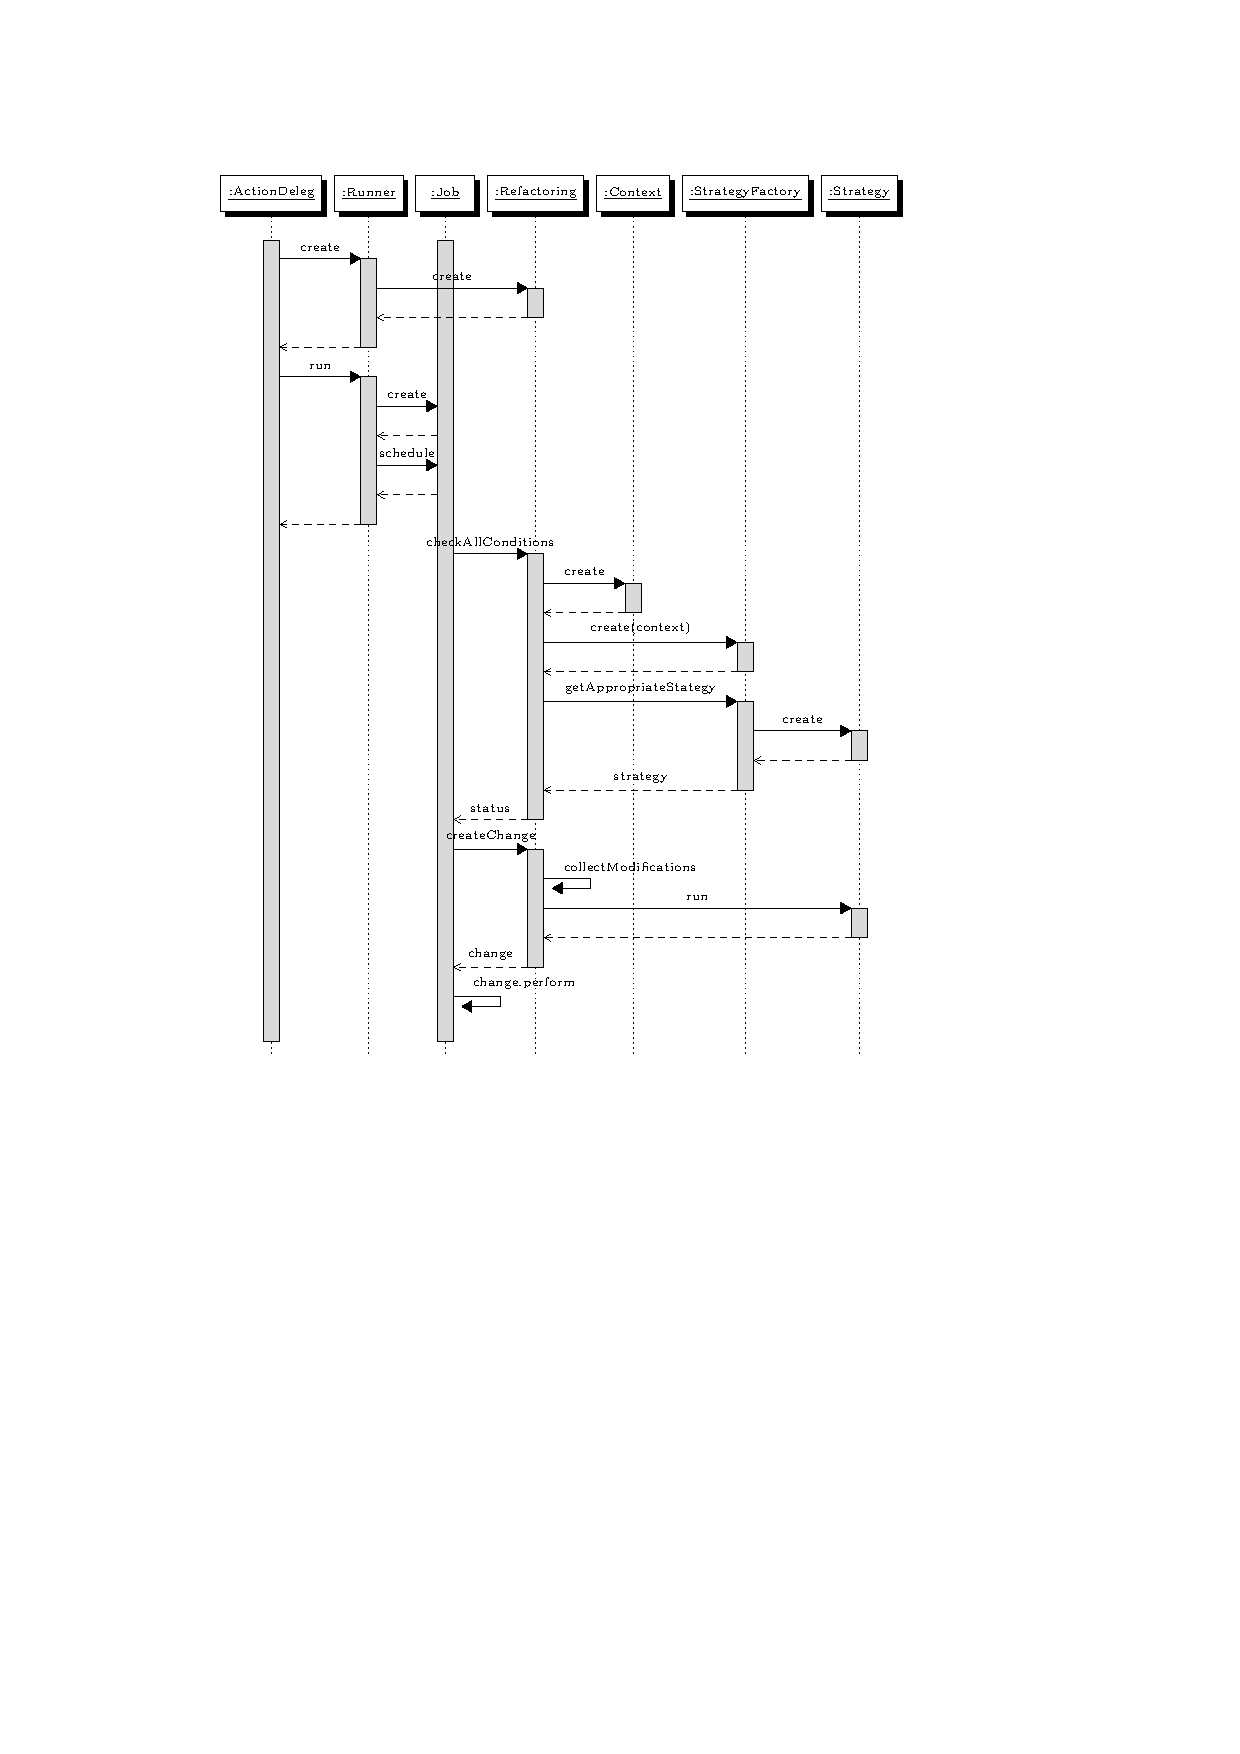
\includegraphics[trim = 35mm 120mm 40mm 28mm,clip,scale=0.8]{seqdiagram/seqdiagram.pdf} %,clip,
  \caption{Basic call flow when toggling a function definition}
  \label{sd}
\end{figure}

\subsection{The strategies}
The \textit{ToggleStrategyFactory} is used to decide which strategy should be 
considered, based on the user selection. The following strategies have been
implemented to cover the specified cases:

\begin{itemize}
\item ToggleFromClassToInHeaderStrategy
\item ToggleFromImplementationHeaderOrClassStrategy
\item ToggleFromInHeaderToClassStrategy
\item ToggleFromInHeaderToImplementationStrategy
\end{itemize}

\subsection{Implications of not using a refactoring wizard}
No wizard was used for this refactoring since it must be fast and may be 
executed several times in succession. When using a wizard, the 
\textit{RefactoringWizardOpenOperation} handles the execution of the refactoring 
inside a separate job. Since the toggle refactoring does not use the wizard, a 
separate job had to be scheduled by the ActionDelegate.

In addition, the undo functionality had to be implemented separately. When the 
changes are performed, they (surprisingly) also return the undo changes that are 
needed by the UndoManager. The UndoManager is available through 
\textit{RefactoringCore.getUndoManager()}. See \textit{ToggleRefactoringRunner} 
for more details on the implementation.

\section{Testing and performance environment}

This section introduces strategies to simplify testing and monitoring of 
performance.

\subsection{A real world test environment}
The COAST~\cite{COAST} source code was used as test environment for real-world 
tests as it uses a lot of C++ code that can be toggled.

\subsection[Fuzzy whitespace recognition for the tests]{Fuzzy whitespace 
recognition for the test environment}

As described in past theses at HSR, the refactoring testing environment
needed an exact definition of the generated code. This was annoying because
same-looking code samples could result in a red bar if white spaces were not the
same. To make writing new tests easier, the comparison method was overridden to
support fuzzy whitespace recognition.

Leading tabs or whitespaces are recognized and it is assumed that the same
indention is used for the whole file. In addition, trailing newlines that are
added by the ASTRewriter are ignored.

The changes made to the CDT test environment help writing new tests without
having to care whether the ASTRewriter uses spaces or tabs for indention.
Resulting code that looks the same now gives a green bar.

\subsection{Testing issues}

The whitespace issue was already discussed. Another issue is that the Doxygen 
syntax //! may not be used in the test files since this syntax is used to 
specify the test name.

\subsubsection{Resource '/RegressionTestProject/A.h' does not exist.}

The following issue was not resolved to its cause and is still active when the 
tests are being run. However, tests still pass without failure. During the test 
run, the following exception is shown on the Eclipse console:

\begin{lstlisting}[language=java]
!ENTRY org.eclipse.cdt.core 4 0 2010-12-13 ...
!MESSAGE Error: Resource '/RegressionTestProject/\
A.h' does not exist.
!STACK 1
org.eclipse.core.internal.resources.\
ResourceException: Resource '/RegressionTest\
Project/A.h' does not exist.
  at...ces.Resource.checkExists(Resource.java:326)
  at...Resource.checkAccessible(Resource.java:200)
  at...l.resources.File.getContents(File.java:291)
  at...aceFileContent(InternalParserUtil.java:145)
  at...ser.FileContent.create(FileContent.java:83)
  at...ser.FileContent.create(FileContent.java:67)
  at...Reader(ProjectIndexerInputAdapter.java:288)
  at...ask.parseFile(AbstractIndexerTask.java:755)
  at....parseLinkage(AbstractIndexerTask.java:688)
  at...rTask.runTask(AbstractIndexerTask.java:343)
  at...OMIndexerTask.run(PDOMIndexerTask.java:127)
  at...PDOMIndexerJob.run(PDOMIndexerJob.java:137)
  at...re.internal.jobs.Worker.run(Worker.java:54)
!SUBENTRY 1 org.eclipse.core.resources 4 368 ...
!MESSAGE Resource '/RegressionTestProject/A.h' \
does not exist.
\end{lstlisting}

\subsubsection{Testing for exceptions}

Error testing is not actually an issue but the mechanism to test for exceptions 
is not obvious, so an example will be shown at this point. 

The .rts test file may include the following syntax:

\begin{lstlisting}[language=java]
//@.config
fatalerror=true
\end{lstlisting}

The \textit{fatalerror} variable may be retrieved using a member function of \textit{RefactoringTest}:
\begin{lstlisting}[language=java]
@Override
protected void configureRefactoring(
    Properties refactoringProperties) {
  fatalError = Boolean.valueOf(
      refactoringProperties.getProperty(
      "fatalerror", "false")).booleanValue();
}
\end{lstlisting}

The \textit{runTest} method may then assert that an error has occurred by using:
\begin{lstlisting}[language=java]
RefactoringStatus initialConditions = 
    refactoring.checkInitialConditions(
    NULL_PROGRESS_MONITOR);
if (fatalError)
  assertConditionsFatalError(initialConditions);
\end{lstlisting}

All in all, the special refactoring test environment developed by \cite{GB06} 
was a big help for refactoring relaxedly.

\subsection{Performance tests}

The simplest way to assess the speed of the refactoring is to look at the junit 
time measurements. The first test that is run takes more time and represents the 
time needed for first time toggling when the refactoring infrastructure has to 
be loaded. 

All performance tests must be executed on the same developer machine, taking the 
average time of three consecutive runs of all tests. Five scenarios have been 
chosen to be able to observe the performance of the toggle refactoring:

\begin{enumerate}
\item First time toggling: Includes loading of the infrastructure and will take 
some more time.
\item Toggle from in class to header: Only one file is affected by this 
refactoring. This represents the least complex refactoring and should be the 
quickest one beside the reference test.
\item Toggle from implementation header: Two files are affected here.
\item Emtpy reference test: A dummy refactoring that won't load and analyze any 
code. Shows what amount of time is consumed by the given refactoring 
infrastructure.
\end{enumerate}

Another technique to measure time more accurately was checked out. For this, the 
\textit{org.eclipse.test.performance} plugin was used. 


